\chapter{Background} \label{Chapter:Background}

This chapter is about the literature review and the brief history of video games that will serve as a valuable background for future research.

\section{A brief history of video games}

It is difficult to tell what counts as the beginning of the video game era. There is a debate about what counts as the very first video game in history. Some consider it to be Tennis for Two (1958)\cite{tennisfortwo1958}, an abstract 2D simulation of tennis played on an oscilloscope. However, the creator, Willy Higinbotham, made Tennis for Two solely to demonstrate the capabilities of the machine it was running on. Therefore, there was no scoring system, nor any other feature that would resemble a modern video game\cite{malliet2005history}.

A better candidate for first place in the history of video games is Spacewar (1962) \cite{spacewar1962}, developed by Steve Russell while he was in college. In contrast with Tennis for Two, Spacewar was intended to be a way of entertainment for two players. It was programmed on PDP-1 mainframe computers and featured a simplified representation of space with two controllable spaceships, a black hole located in the middle of the screen, and a few blinking stars to decorate the screen. The task for the two players was to destroy the other's spaceship by firing torpedoes at it while avoiding crashing into the black hole. Since Spacewar was a computer program intentionally developed for entertainment, it is safe to say that it was the first true video game. Furthermore, it established the foundations of the action and simulation genres that emerged shortly after\cite{malliet2005history}.



\section{Defining video game genres}

The first attempts to classify video games occurred years after the first video game was released. In his book released in 1984, Chris Crawford listed games in two major categories, namely skill and action games (S\&A) which rely heavily on hand-eye coordination and motor skills and are usually fast-paced, and strategy games that emphasize more decision-making, and due to their nature, they generally take longer than S\&A games\cite{crawford1984art}. Within these main categories, Crawford defined multiple subdivisions for finer categorization. Some of these categories have evolved into modern game genres and are still present today, like sports and adventure games, while others, including paddle games, D\&D games and games of chance have completely merged into other genres and do not exist on their own. It is important to note that Crawford did not refer to these categories as genres.

Many of the first definitions of true video game genres were formulated by Mark J. P. Wolf, who also compared video games with the other existing media types, but mainly cinema \cite{wolf2002genre}. He concluded that video games and movies, while many similarities exist, can not be categorized the same way, due to their differences in interactivity (video games require active participation from the audience). Thus, the 41 genres and subgenres explained in his paper\cite{wolf2002genre} are based on interactivity aspects, instead of iconography. The border between some of these genres is blurry, Racing and Driving, Catching and Capturing, Obstacle Course, and Platform all have a surprisingly similar definition to the other, differing only in a few parameters; however, these similarities are explicitly stated by the author.

Another approach was made in 2006 by Thomas H. Apperley, who agreed with Wolf that games cannot be categorized like other media types. He also criticized earlier game categorization attempts, mainly because they are "loose aesthetic clusters based around video games' aesthetic linkages to prior media forms"\cite{apperley2006genre}. Instead, his proposed framework tries to shape a new set of genres around the style of "ergodic interaction" that takes place within the games. In his paper, he defined four distinct video game genres. \textit{Simulation} games mimic the intricate processes of real-life systems, such as cars or cities. \textit{Strategy} games, including real-time strategy (RTS) and turn-based strategy (TBS), are outliers due to their similarity to board games. These games usually have a god's-eye view and information-heavy interfaces. \textit{Action} games include first-person shooters (FPS) and third-person games and focus more on the player's performance in combat manoeuvres and aiming with weapons, and unlike strategy games, they do not contain complex decision-making processes. And finally, \textit{role-playing} games (RPG), often compared to pencil-and-paper RPGs like Dungeons and Dragons, usually revolve around fantasy themes and focus on some form of character development, such as the collection of experience or skill points.

The early video game taxonomies were not applicable to the modern genres that followed\cite{starosta2024tangled}. Such complex genres as Massively Multiplayer Online Role-Playing Games (MMORPG) or Multiplayer Online Battle Arenas (MOBA) could not fit into the existing categories that were shaped, as they are a mix of several already defined game types (Multiplayer and Role-Playing).

Overall, it can be observed that the video game industry is and has always been struggling to come up with a universal organization system for games. Existing categorization methods, such as those used for books or movies, could not be applied due to differences between the mediums\cite{lee2014facet}.

Instead of sticking to one taxonomy, Steam\cite{steam}, an online video game store, uses a list of predefined, as well as user-defined, tags (consisting of one or a few words) to categorize games published on the platform. Tags are similar, and sometimes identical, to the name of genres discussed in the above-mentioned papers, however, there is no definition linked to them. What each tag means is determined by the types of games assigned to them on the platform. This enables a greater freedom in video game categorization than sicking to a chosen taxonomy would, since tags can expand and adapt to new game types, while taxonomies remain the same.



\section{Genre combinations}

In 1993, Doom\cite{doom1993} was released, a prime example of a genre being born. Even though Doom was not the first of its kind, and just like other games, it was a combination of already existing genres like action and shooter, it became so successful and popular that the common term to describe similar games became "doom-clone". Only a couple of years later did a proper name "first-person shooter" (FPS) for these types of games appear and gain mass acceptance\cite{arsenault2009}, thus giving birth to a new video game genre.

Soulslike games share a similar story, although 'Soulslike' is not considered a genre of its own but rather a subgenre. Its name comes from games developed by FromSoftware, a game development studio that is mainly famous for its games of high difficulty, namely Demon's Souls and the Dark Souls trilogy, all built around a very similar theme and game aesthetics, dynamics and mechanics\cite{hunicke2004mda}. Since these games are relatively new (the oldest, Demon's Souls, was released in 2009), a better and more descriptive name for this sub-genre has not been found yet.



\section{Finding genre combinations}

Today's most popular game store on PC, Steam\cite{steam}, which, at the time of writing, has a library of over 204.000 apps, including the majority of modern video games. There are some exceptions, however, as some games are platform-specific and thus have never been released on Steam, but the number of such games can only be measured in the hundreds, so they will be considered insignificant for this research.

Steam uses two systems to categorize this massive amount of content. First, developers and publishers pick from a list of pre-defined genres to assign to their apps during upload. Second, users who download these apps can assign them user-defined tags that can indicate genre, theme, aesthetic or even difficulty, and help other users find new apps that are to their liking. From the user's point of view, only the tags are visible on the apps' dedicated pages while genres are only used as filtering in the store's search field.

Steam has a public API (Application Programming Interface) that can be used to query data about their games and apps. This API, however, is not well-documented, thus it would take a considerable amount of trial and error to use it properly. Luckily, a relatively fresh dataset\cite{steamCatalogInsight2024} can be found on GitHub that, according to the author, was acquired in October 2024 using the Steam API and contains all the data necessary to find existing genre combinations on Steam. To check exactly how up-to-date this data set is, I checked the number of games under some tags on Steam and compared them to the numbers found in the data set, and the differences were around 40\%, which is unexpectedly high. However, games released in October 2024 can be found in the data set as expected with the correct release dates, indicating the data was truly acquired in or after October 2024. The explanation for such a large difference in the numbers could be explained by the ever-rising number of new games published each month on the platform, and the new tags applied to games during this two-month period. However, the ratio between the tag occurrences could not change significantly under such a short time. These data are in CSV format which is mostly used by spreadsheet editors such as Excel or Numbers, but can easily be read from script too.

Going through the data set and individually counting the times each tag occurs, it is easy to determine that Steam currently uses 447 tags and 121 genres. It can also be observed that tag occurrences, as seen in the figure \ref{figure:tags}, like many other data sets, seem to follow Zipf's law loosely\cite{li2002zipf}. Interestingly, some of the tags make little sense, like "Intentionally Awkward Controls" or "TrackIR", and do not represent a genre, but rather some other aspect of the game. There are a few tags like "Warhammer 40K" that solely indicate which franchise the game belongs to.

\begin{figure}[h]
    \centering
    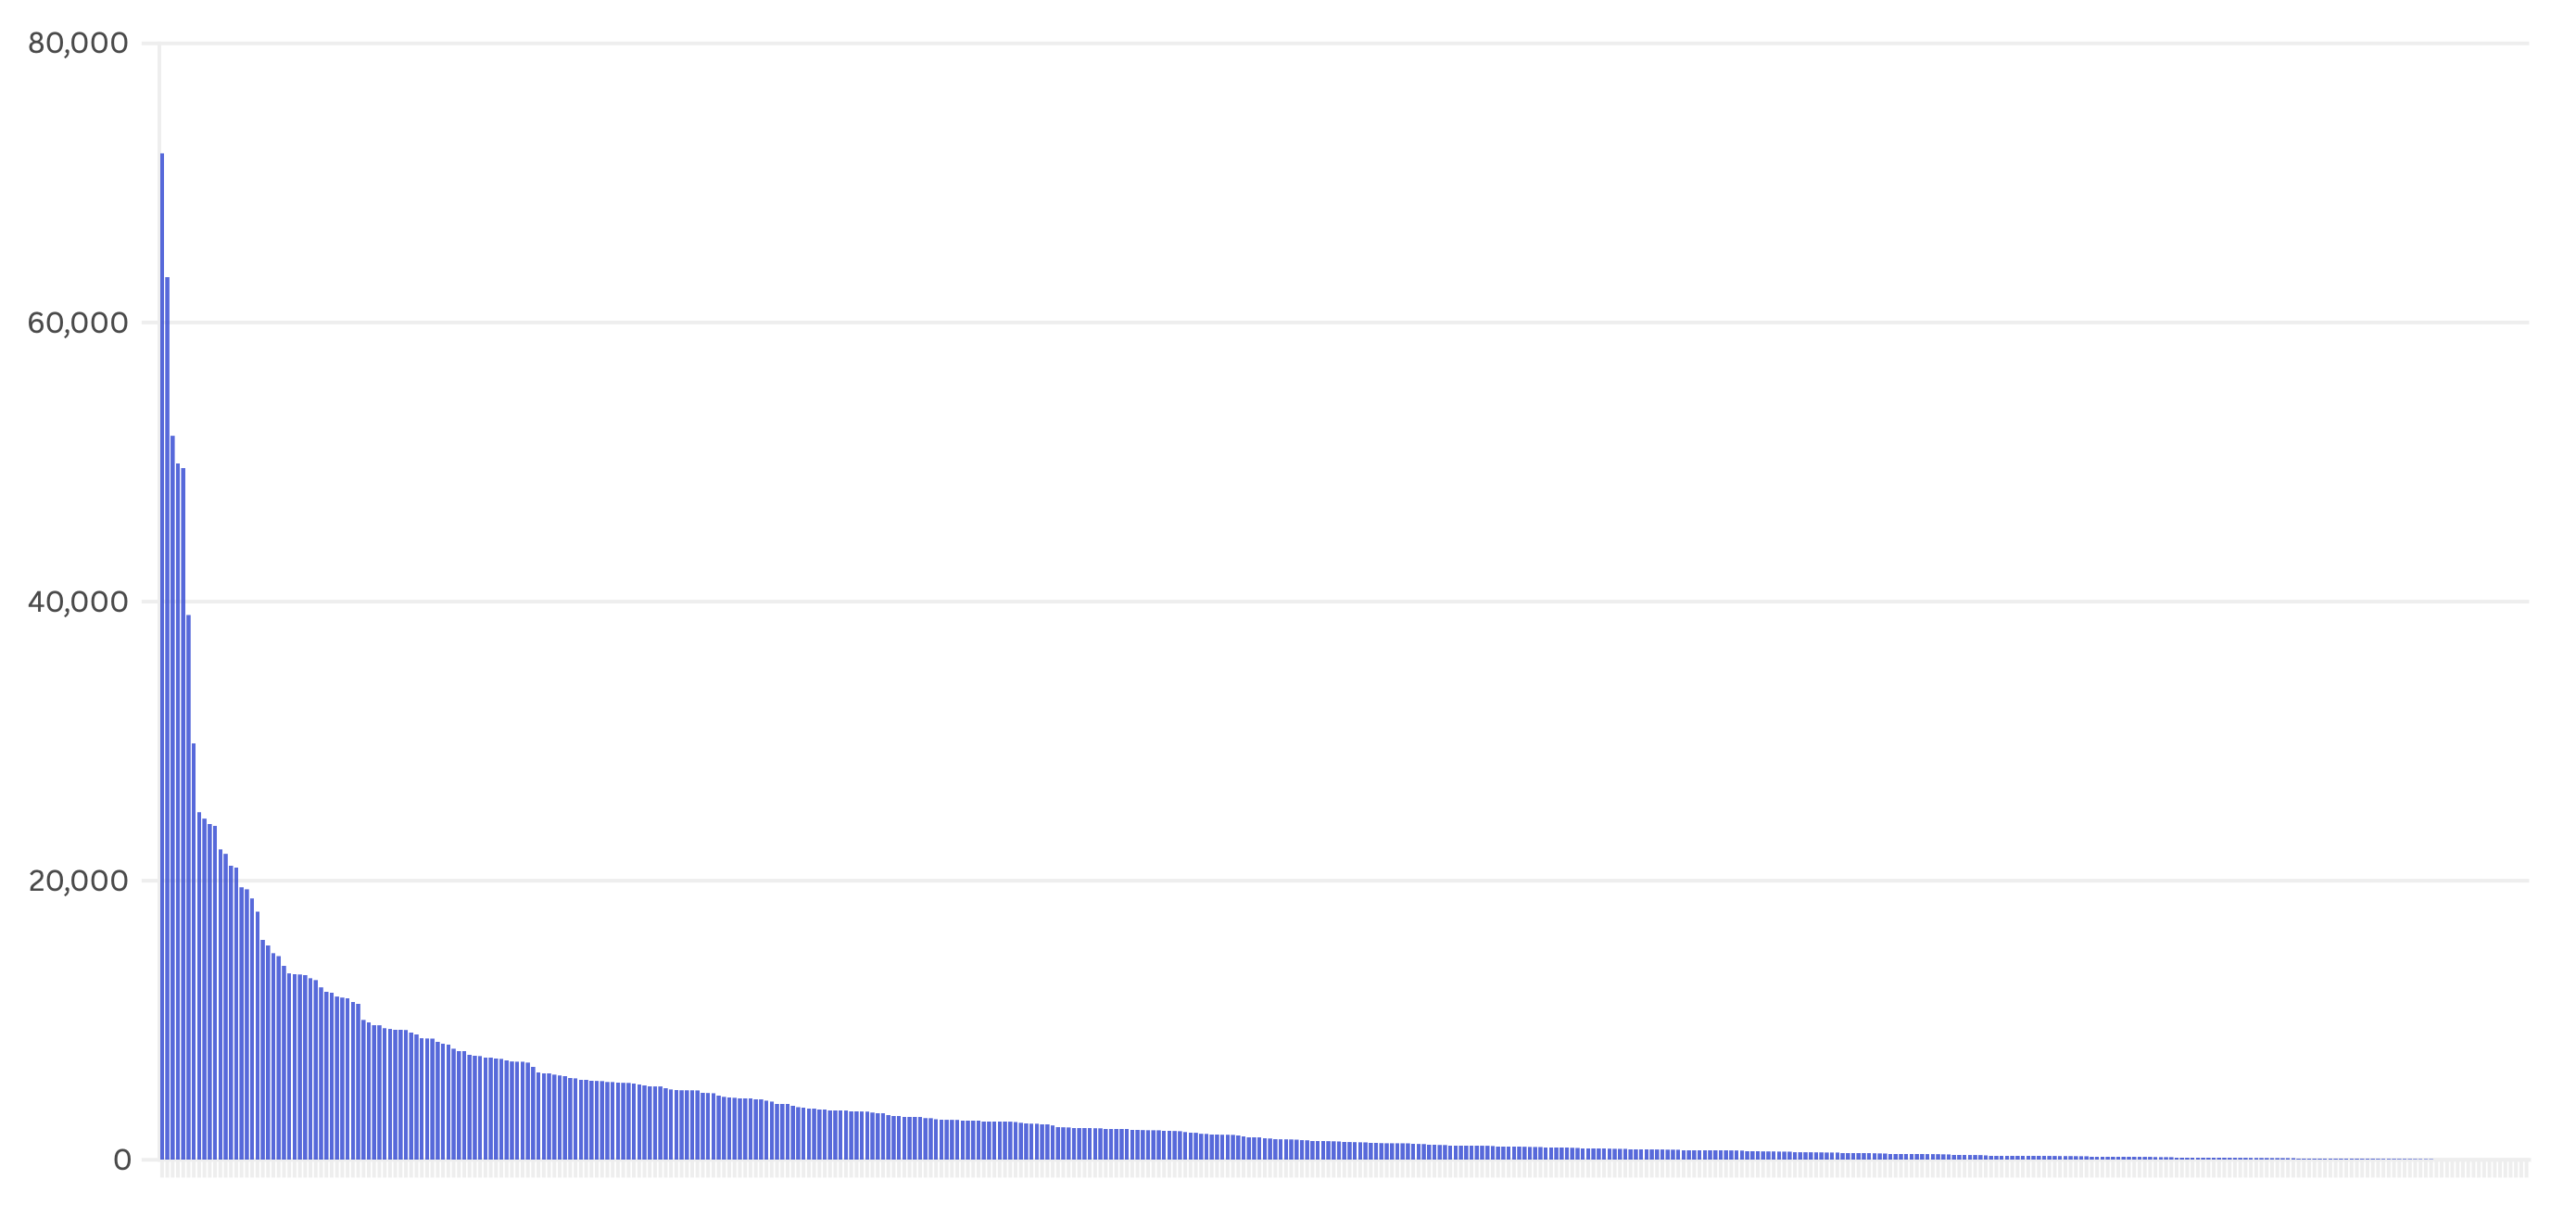
\includegraphics[width=\textwidth]{images/tag-occurrences.png}
    \caption{Tag occurrences}
    \label{figure:tags}
\end{figure}

On the other hand, the genre distribution in figure \ref{figure:genres} seems unbalanced. The reason for that is that for some reason, 84 of the 121 genres are localized versions of others, and each appears less than 30 times. These genres can be safely discarded, as their occurrence times would not contribute too much to the other numbers.

\begin{figure}[h]
    \centering
    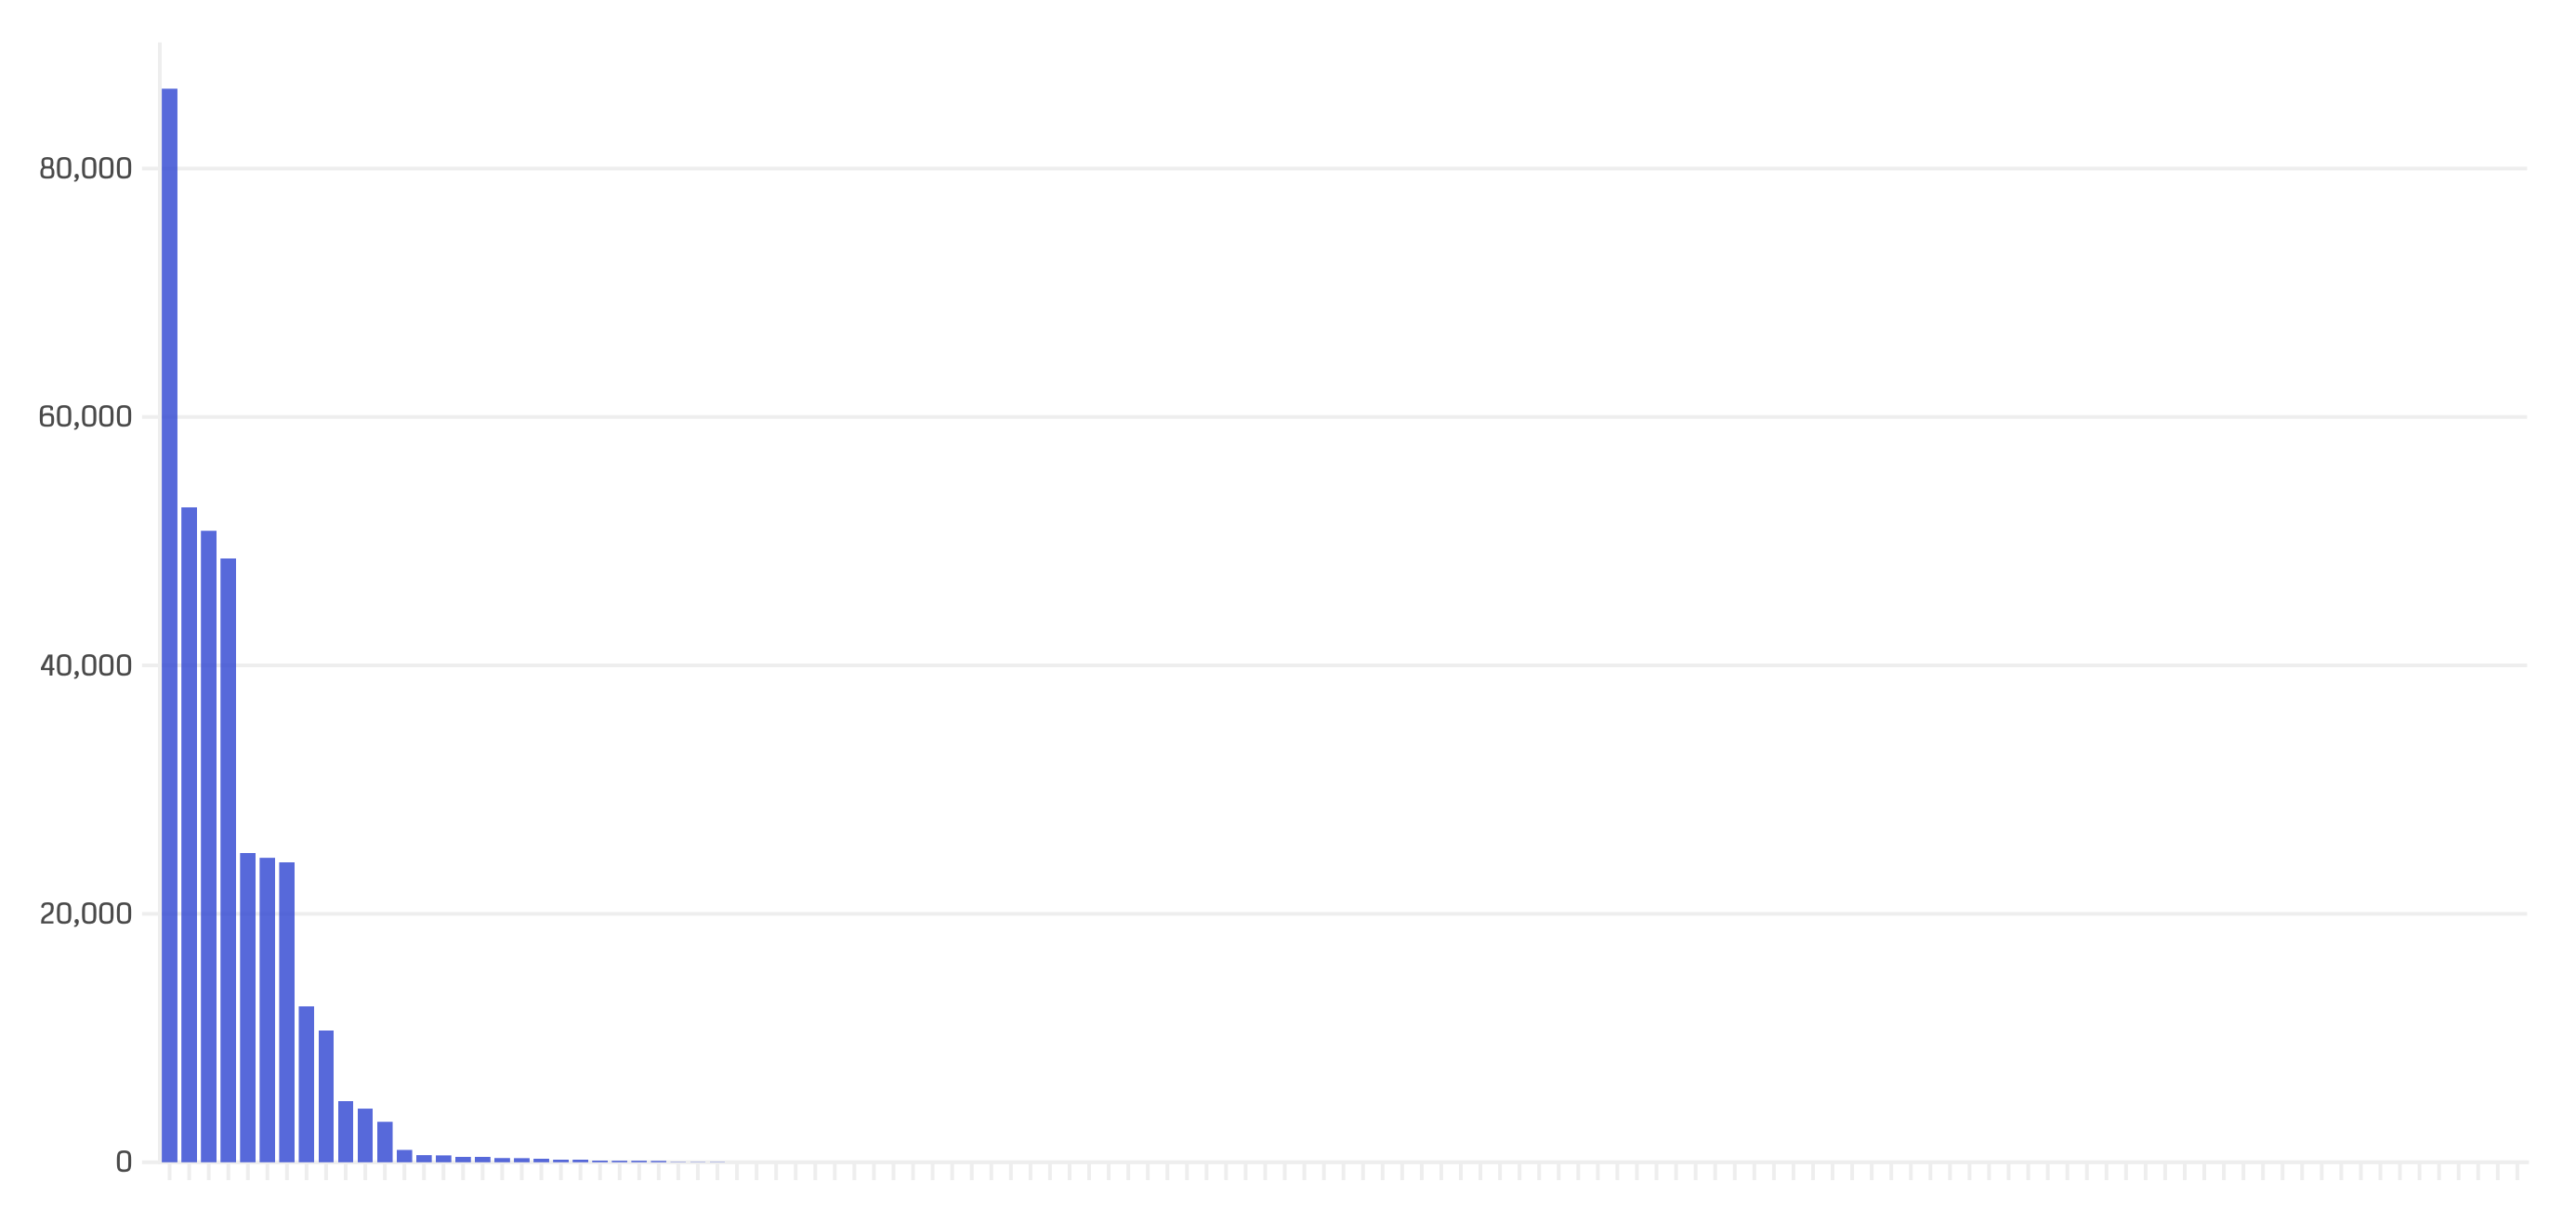
\includegraphics[width=\textwidth]{images/genre-occurrences.png}
    \caption{Genre occurrences}
    \label{figure:genres}
\end{figure}

However, since Steam uses only a handful of genres to categorize games, these genres are vague. Therefore, for this thesis, I will use Steam tags instead, as tags provide a much finer way to describe what genres the developed game prototype should belong to, and what types of game mechanics they use.

It is important to note that the dataset's author also looked for genre combinations as seen in figure \ref{figure:genre-pairs}, but they only used combinations of two genres, while I was more interested in more complex mixtures. Furthermore, they only included tags assigned to at least 900 games in the Steam library, and that criteria takes away almost half of the tags. For this thesis, I am interested in the other half of the tags, those that are used very rarely, but at the same time, clearly represent a genre or sub-genre. To extract exactly the data I needed, I had to write my own script.

\begin{figure}[h]
    \centering
    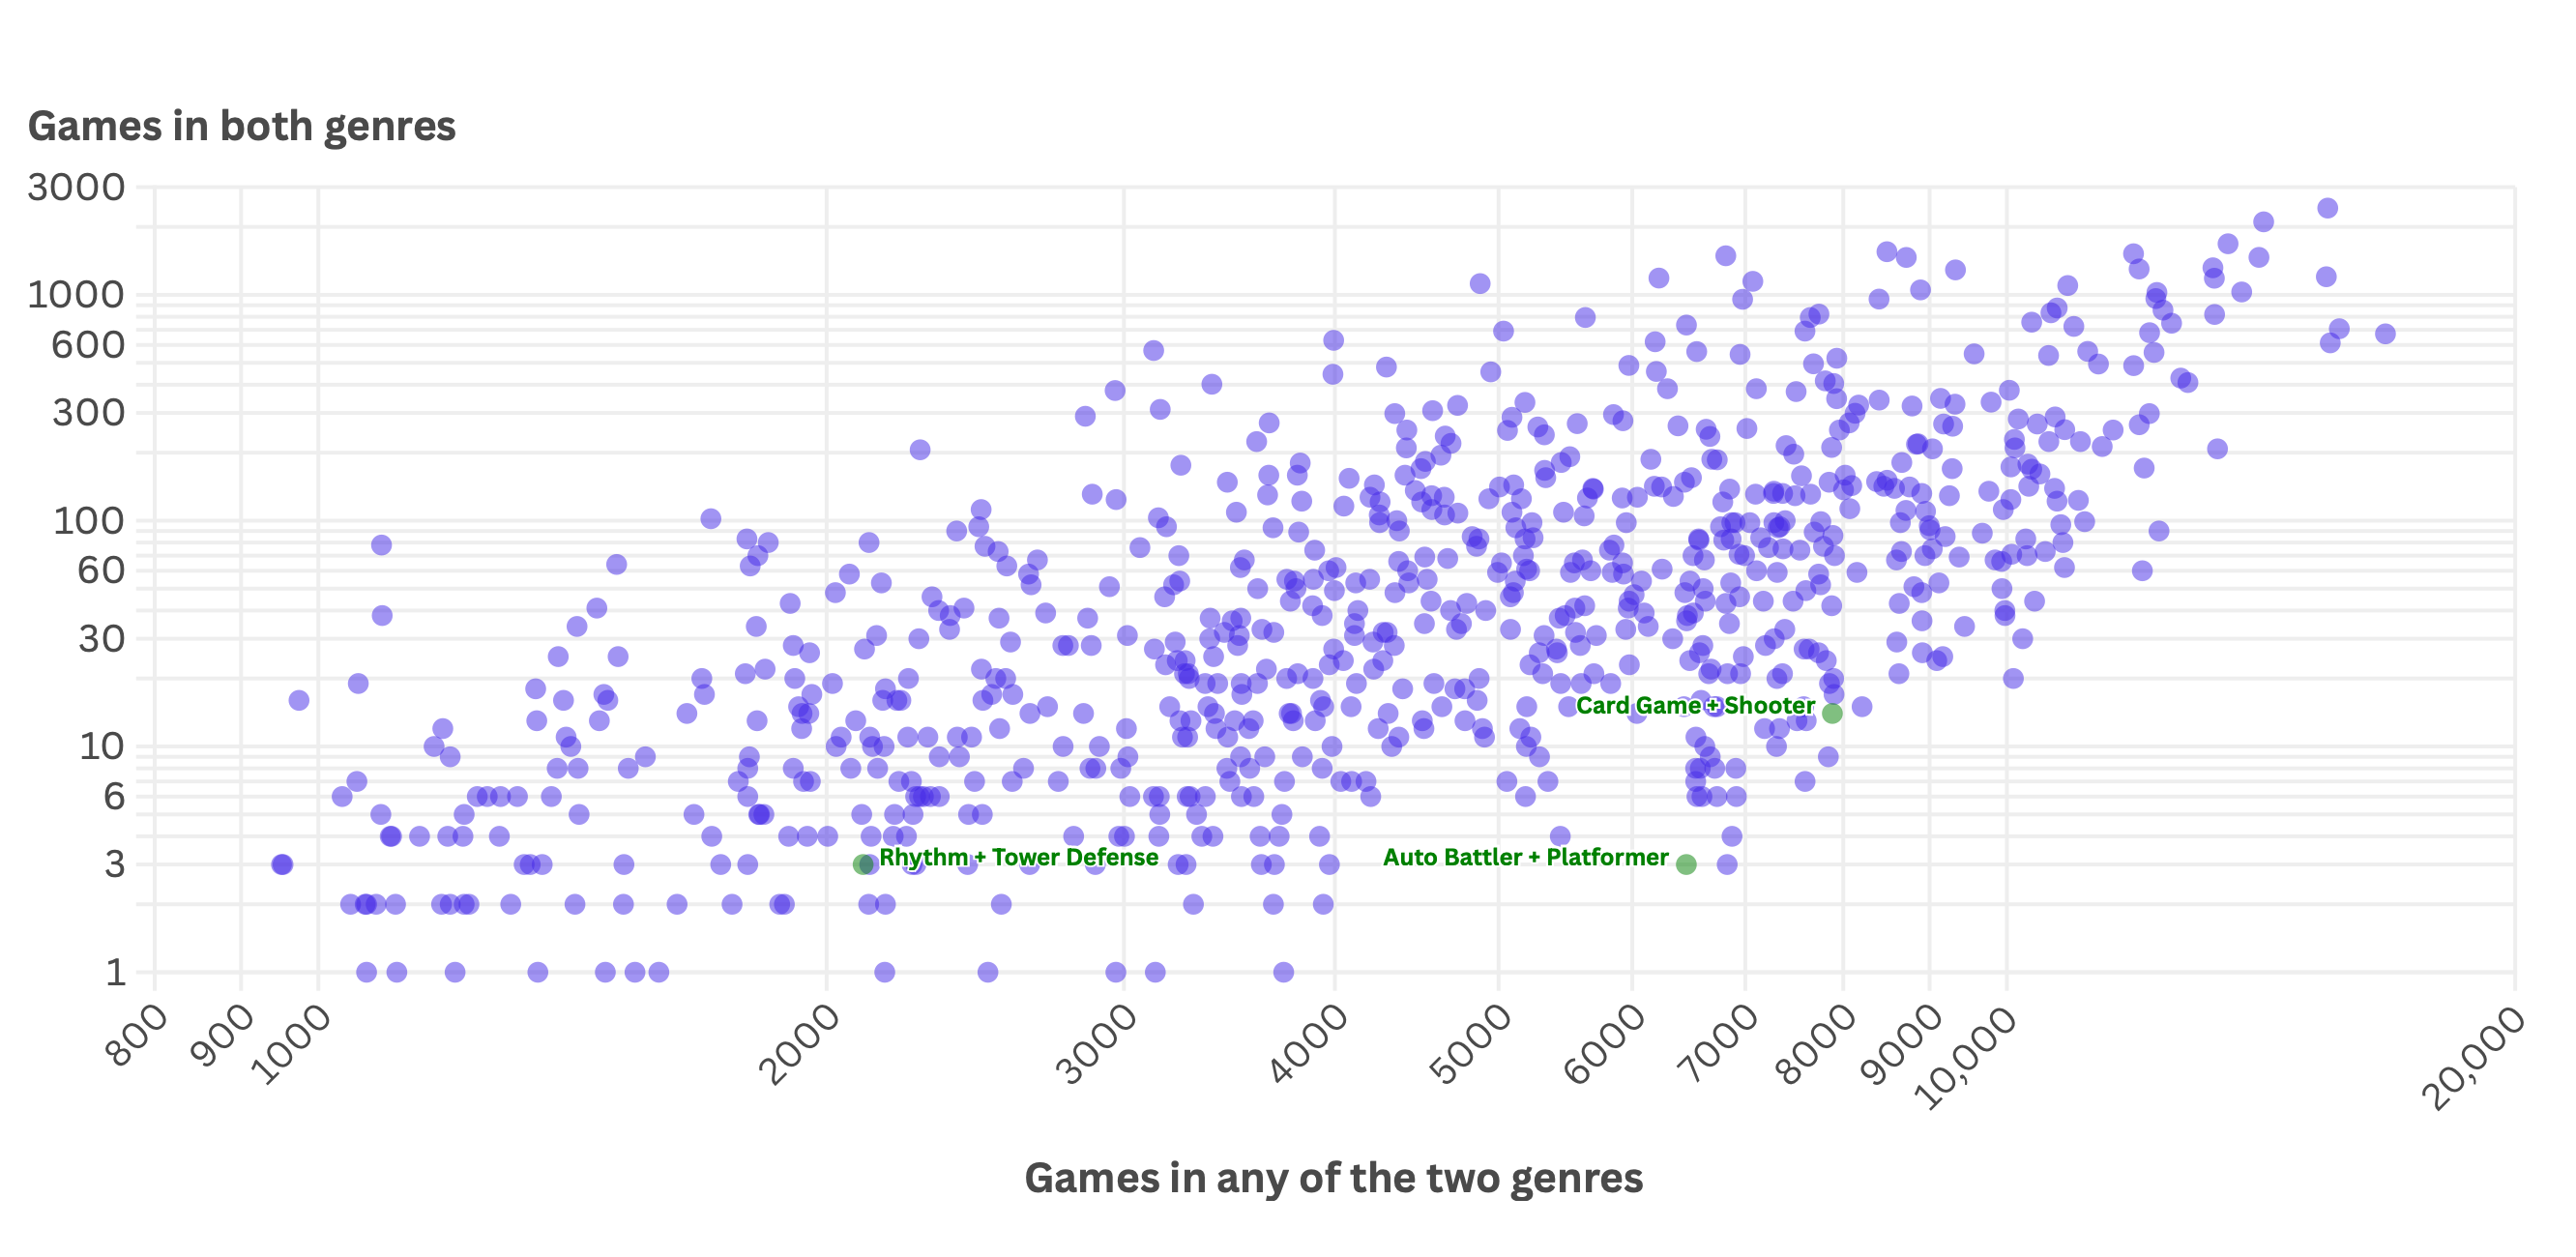
\includegraphics[width=\textwidth]{images/genre-pairs.png}
    \caption{Most frequent genre pairs}
    \label{figure:genre-pairs}
\end{figure}



\section{Game engines}

This thesis will include the development of a game prototype, and to reduce development time, a game engine will be used. There are many freely available game engines on the market at the time this thesis is being written, so to pick one, a short comparison needs to be made.

But first of all, what is a game engine? To answer this question, it would be a good idea to look back at the very first game engine. Doom Engine was developed for Doom (1993) by id Software, it was the first of its kind \cite{gregory2018gameEngineArchitecture}, the very first piece of software that had its components well-defined and separated, allowing developers to make different games with minimal modifications made to the game engine itself. Soon many major game development studios started to develop their own game engines, while licensing other's already working engines started to become a norm.

% Expand, and move the below section to methods

Today, developers have even more options, as (initially) free-to-use and open-source Game Engines have become very popular, such as Unity, Unreal Engine (UE) and Godot. Out of these three, only Godot is truly free to use, as the other two do require a share of the game's total revenue to be paid if that reaches a certain limit. Furthermore, Godot also seems to be the optimal choice for this thesis, since it is much more lightweight and more user-friendly than the others.

Godot uses its own scripting language called GDScript, which is very similar to Python. However, there is an option to use C\# instead, a much more widely used language, in Godot's Mono (.NET) version.


% Theory: find sikilar papers